\documentclass{article}
\usepackage{amsfonts}
\usepackage{amsmath}
\usepackage{amssymb}
\usepackage{hyperref}
\usepackage{mathrsfs}
\usepackage{tikz}

\parindent=0pt

\usetikzlibrary{positioning}

\def\upint{\mathchoice%
    {\mkern13mu\overline{\vphantom{\intop}\mkern7mu}\mkern-20mu}%
    {\mkern7mu\overline{\vphantom{\intop}\mkern7mu}\mkern-14mu}%
    {\mkern7mu\overline{\vphantom{\intop}\mkern7mu}\mkern-14mu}%
    {\mkern7mu\overline{\vphantom{\intop}\mkern7mu}\mkern-14mu}%
  \int}
\def\lowint{\mkern3mu\underline{\vphantom{\intop}\mkern7mu}\mkern-10mu\int}

\begin{document}

\textbf{\Large Chapter 2: Modules} \\\\



\emph{Author: Meng-Gen Tsai} \\
\emph{Email: plover@gmail.com} \\\\



% https://metaphor.ethz.ch/x/2018/hs/401-3132-00L/ex/sol_4.pdf



\textbf{Exercise 2.1}
\emph{Show that
$(\mathbb{Z}/m\mathbb{Z}) \otimes_{\mathbb{Z}} (\mathbb{Z}/n\mathbb{Z}) = 0$
if $m$, $n$ are coprime.} \\

It suffices to show that
$$(\mathbb{Z}/m\mathbb{Z}) \otimes_{\mathbb{Z}} (\mathbb{Z}/n\mathbb{Z})
\cong \mathbb{Z}/d\mathbb{Z}$$
where $d$ is the greatest common divisor of $m$ and $n$. \\

\emph{Outlines.}
\begin{enumerate}
\item[(1)]
Define $\widetilde{\varphi}$ by
\begin{center}
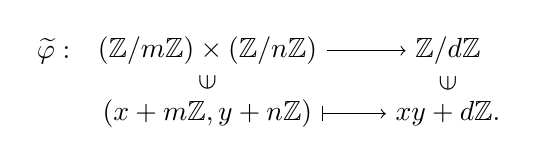
\begin{tikzpicture}[node distance=1mm]
  \node (functionName) at (0, 0) {$\widetilde{\varphi}:$};
  \node[right = of functionName] (domain)
    {$(\mathbb{Z}/m\mathbb{Z}) \times (\mathbb{Z}/n\mathbb{Z})$};
  \node[below = 2mm of domain] (element) {$(x + m\mathbb{Z}, y + n\mathbb{Z})$};
  \path (element)--(domain)node[midway,sloped] {$\in$};
  \node[right = 1cm of domain] (codomain) {$\mathbb{Z}/d\mathbb{Z}$};
  \node at (element-|codomain) (image) {$xy + d\mathbb{Z}.$};
  \path (image)--(codomain)node[midway,sloped] {$\in$};
  \draw[->] (domain) -- (codomain);
  \draw[|->] (element) -- (image);
\end{tikzpicture}
\end{center}
$\widetilde{\varphi}$ is well-defined and $\mathbb{Z}$-bilinear.
\item[(2)]
By the universal property,
$\widetilde{\varphi}$ factors through a $\mathbb{Z}$-linear map
$$\varphi: (\mathbb{Z}/m\mathbb{Z}) \otimes_{\mathbb{Z}} (\mathbb{Z}/n\mathbb{Z})
\rightarrow \mathbb{Z}/d\mathbb{Z}$$
(such that $\varphi(x \otimes y) = \widetilde{\varphi}(x, y)$).
\item[(3)]
To show that $\varphi$ is isomorphic, might find the inverse map
$\psi: \mathbb{Z}/d\mathbb{Z}
\rightarrow
(\mathbb{Z}/m\mathbb{Z}) \otimes_{\mathbb{Z}} (\mathbb{Z}/n\mathbb{Z})$
of $\varphi$.
Define $\psi$ by
\begin{center}
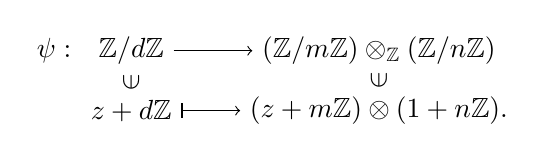
\begin{tikzpicture}[node distance=1mm]
  \node (functionName) at (0, 0) {$\psi:$};
  \node[right = of functionName] (domain) {$\mathbb{Z}/d\mathbb{Z}$};
  \node[below = 2mm of domain] (element) {$z + d\mathbb{Z}$};
  \path (element)--(domain)node[midway,sloped] {$\in$};
  \node[right = 1cm of domain] (codomain)
    {$(\mathbb{Z}/m\mathbb{Z}) \otimes_{\mathbb{Z}} (\mathbb{Z}/n\mathbb{Z})$};
  \node at (element-|codomain) (image) {$(z + m\mathbb{Z}) \otimes (1 + n\mathbb{Z}).$};
  \path (image)--(codomain)node[midway,sloped] {$\in$};
  \draw[->] (domain) -- (codomain);
  \draw[|->] (element) -- (image);
\end{tikzpicture}
\end{center}
$\psi$ is well-defined and $\mathbb{Z}$-linear.
\item[(4)]
$\psi \circ \varphi = \text{id}$.
\item[(5)]
$\varphi \circ \psi = \text{id}$. \\
\end{enumerate}

\emph{Proof of (1).}
\begin{enumerate}
\item[(a)]
\emph{$\widetilde{\varphi}$ is well-defined.}
Say $x' = x + am$ for some $a \in \mathbb{Z}$
and $y' = y + bn$ for some $b \in \mathbb{Z}$.
Then $x'y' - xy = yam + xbn + abmn \in \mathbb{Z}/d\mathbb{Z}$.
That is, $\widetilde{\varphi}$
is independent of coset representative.
\item[(b)]
\emph{$\widetilde{\varphi}$ is $\mathbb{Z}$-bilinear.}
\begin{enumerate}
\item[(i)]
\emph{For any $\lambda \in \mathbb{Z}$,
$\widetilde{\varphi}(\lambda x, y)
= \widetilde{\varphi}(x, \lambda y)
= \lambda \widetilde{\varphi}(x, y)$.}
In fact,
\begin{align*}
  \widetilde{\varphi}(\lambda(x+m\mathbb{Z}), y+n\mathbb{Z})
  &= \widetilde{\varphi}(\lambda x+m\mathbb{Z}, y+n\mathbb{Z})
  = \lambda x y + d\mathbb{Z}, \\
  \widetilde{\varphi}(x+m\mathbb{Z}, \lambda(y+n\mathbb{Z}))
  &= \widetilde{\varphi}(x+m\mathbb{Z}, \lambda y+n\mathbb{Z})
  = \lambda x y + d\mathbb{Z}, \\
  \widetilde{\varphi}(x_1+m\mathbb{Z}, y+n\mathbb{Z})
  &= \lambda (x y + d\mathbb{Z})
  = \lambda x y + d\mathbb{Z}.
\end{align*}
\item[(ii)]
\emph{$\widetilde{\varphi}(x_1 + x_2, y)
= \widetilde{\varphi}(x_1, y) + \widetilde{\varphi}(x_2, y)$.}
In fact,
\begin{align*}
  \widetilde{\varphi}((x_1+x_2)+m\mathbb{Z}, y+n\mathbb{Z})
  &= (x_1 + x_2) y + d\mathbb{Z}, \\
  \widetilde{\varphi}(x_1+m\mathbb{Z}, y+n\mathbb{Z})
  + \widetilde{\varphi}(x_2+m\mathbb{Z}, y+n\mathbb{Z})
  &= (x_1 y + d\mathbb{Z}) + (x_2 y + d\mathbb{Z}) \\
  &= (x_1 + x_2) y + d\mathbb{Z}.
\end{align*}
\item[(iii)]
\emph{$\widetilde{\varphi}(x, y_1 + y_2)
= \widetilde{\varphi}(x, y_1) + \widetilde{\varphi}(x, y_2)$.}
Similar to (ii).
\end{enumerate}
\end{enumerate}
$\Box$ \\

\emph{Proof of (3).}
\begin{enumerate}
\item[(a)]
\emph{$\psi$ is well-defined.}
Say $z' = z + cd$ for some $c \in \mathbb{Z}$.
Note that $d = \alpha m + \beta n$ for some $\alpha, \beta \in \mathbb{Z}$.
Thus
\begin{align*}
  \psi(z' + d\mathbb{Z})
  &= \psi(z + cd + d\mathbb{Z}) \\
  &= \psi(z + c(\alpha m + \beta n) + d\mathbb{Z}) \\
  &= (z + c(\alpha m + \beta n) + m\mathbb{Z}) \otimes (1 + n\mathbb{Z}) \\
  &= (z + c \beta n + m\mathbb{Z}) \otimes (1 + n\mathbb{Z}) \\
  &= (z + m\mathbb{Z}) \otimes (1 + n\mathbb{Z})
  + (c \beta n + m\mathbb{Z}) \otimes (1 + n\mathbb{Z}) \\
  &= \psi(z + d\mathbb{Z})
  + (1 + m\mathbb{Z}) \otimes (c \beta n + n\mathbb{Z}) \\
  &= \psi(z + d\mathbb{Z}).
\end{align*}
\item[(b)]
\emph{$\psi$ is $\mathbb{Z}$-linear.} For any $\lambda \in \mathbb{Z}$,
\begin{align*}
  \psi(\lambda(z + d\mathbb{Z}))
  &= \psi(\lambda z + d\mathbb{Z})
  = (\lambda z + m\mathbb{Z}) \otimes (1 + n\mathbb{Z}), \\
  \lambda \psi(z + d\mathbb{Z})
  &= \lambda((z + m\mathbb{Z}) \otimes (1 + n\mathbb{Z}))
  = (\lambda z + m\mathbb{Z}) \otimes (1 + n\mathbb{Z}).
\end{align*}
\end{enumerate}
Thus, $\psi(\lambda z) = \lambda \psi(z)$.
$\Box$ \\

\emph{Proof of (4).}
For any $(x + m\mathbb{Z}) \otimes (y + n\mathbb{Z}) \in
(\mathbb{Z}/m\mathbb{Z}) \otimes_{\mathbb{Z}} (\mathbb{Z}/n\mathbb{Z})$,
\begin{align*}
  \psi(\varphi((x + m\mathbb{Z}) \otimes (y + n\mathbb{Z})))
  &= \psi(xy + d\mathbb{Z}) \\
  &= (xy + m\mathbb{Z}) \otimes (1 + n\mathbb{Z}) \\
  &= (x + m\mathbb{Z}) \otimes (y + n\mathbb{Z}).
\end{align*}
$\Box$ \\

\emph{Proof of (5).}
For any $z + d\mathbb{Z} \in \mathbb{Z}/d\mathbb{Z}$,
\begin{align*}
  \varphi(\psi(z + d\mathbb{Z})
  &= \varphi((z + m\mathbb{Z}) \otimes (1 + n\mathbb{Z})) \\
  &= z + d\mathbb{Z}.
\end{align*}
$\Box$ \\\\



\end{document}